\documentclass[english]{article}

%% Packages pull in extra commands:
%% http://en.wikibooks.org/wiki/LaTeX/Packages
\usepackage[latin9]{inputenc}
\usepackage[letterpaper]{geometry}
\geometry{verbose,tmargin=1in,bmargin=1in,lmargin=1in,rmargin=1in}
\usepackage{amsmath}
\usepackage{amssymb}
\usepackage{graphicx}
\usepackage{float}
\usepackage{array}
\usepackage{tikz}
\usepackage{latexsym}
\usepackage{xspace}
\usepackage{float}
\restylefloat{table}

% New commands serve as shorthand for frequently used command combinations.
\newcommand{\ind}[1]{\mathbf{1}\left(#1\right)}
\newcommand{\bx}{\mathbf{x}}
\newcommand{\E}{\mathbf{E}}
\newcommand{\bw}{\mathbf{w}}
\renewcommand{\Pr}{\mathbf{Pr}\xspace}
\newcommand{\Bern}{\textsf{Bernoulli}\xspace}
\newcommand{\XX}{\mathcal{X}}

\title{CIS 520, Machine Learning, Fall 2015: Assignment 3}
\author{Arpit Panwar}

\begin{document}
\maketitle
{\normalsize Collaborator: \\ 
\\ \underline{ Anusha Fernando }

\section{Linear Regression and LOOCV}

%\newcommand{\bw}{\mathbf{w}}

In the last homework, you learned about using cross validation as a
way to estimate the true error of a learning algorithm.  A solution
that provides an almost unbiased estimate of this true error is
\emph{Leave-One-Out Cross Validation} (LOOCV), but it can take a
really long time to compute the LOOCV error.  In this problem, you
will derive an algorithm for efficiently computing the LOOCV error for
linear regression using the \emph{Hat Matrix}.
\footnote{Unfortunately, such an efficient algorithm may not
be easily found for other learning methods.}

Assume that there are $n$ given training examples,
$(X_1,Y_1),(X_2,Y_2),\dots,(X_n,Y_n)$, where each input data point
$X_i$, has $m$ real-valued features.  The goal of regression is to
learn to predict $Y$ from $X$.  The \emph{linear} regression model
assumes that the output $Y$ is a weighted \emph{linear} combination of
the input features with weights given by $\bw$, plus some Gaussian
noise.

We can write this in matrix form by stacking the data points as the
rows of a matrix $X$ so that $x_{ij}$ is the $j$-th feature of the
$i$-th data point.  Then writing $Y$, $\bw$ and $\epsilon$ as column
vectors, we can express the linear regression model in matrix form as
follows:

\[
Y=X\bw + \epsilon
\]

where:

\[
Y = \left[\begin{array}{c}
Y_1 \\
Y_2 \\
\vdots \\
Y_n
\end{array}\right],
X = \left[\begin{array}{cccc}
x_{11} & x_{12} & \dots & x_{1m} \\
x_{21} & x_{22} & \dots & x_{2m} \\
\vdots & \vdots & \ddots & \vdots \\
x_{n1} & x_{n2} & \dots & x_{nm} \\
\end{array}\right],
\bw = \left[\begin{array}{c}
w_1 \\
w_2 \\
\vdots \\
w_m
\end{array}\right],
\,\,\,\,\,\mbox{and}\,\,
\epsilon = \left[\begin{array}{c}
\epsilon_1 \\
\epsilon_2 \\
\vdots \\
\epsilon_n
\end{array}\right]
\]
Assume that $\epsilon_i$ is normally distributed with variance
$\sigma^2$.  We saw in class that the maximum likelihood estimate of
the model parameters $\bw$ (which also happens to minimize the sum of
squared prediction errors) is given by the \emph{Normal equation}:
\[
\hat{\bw} = (X^TX)^{-1} X^TY
\]

\noindent Define $\hat{Y}$ to be the vector of predictions using
$\hat{\bw}$ if we were to plug in the original training set $X$:
\begin{eqnarray*}
\hat{Y} &=& X\hat{\bw}  \\
    &=& X(X^T X)^{-1} X^T Y \\
    &=& H Y
\end{eqnarray*}
where we define $H=X(X^T X)^{-1} X^T$ ($H$ is often called the
\emph{Hat Matrix}).

\noindent As mentioned above, $\hat{\bw}$, also minimizes the sum of
squared errors:
\[
\mbox{SSE} = \sum_{i=1}^{n} (Y_i-\hat{Y}_i)^2
\]
Now recall that the Leave-One-Out Cross Validation score is defined to
be:
\[
\mbox{LOOCV} = \sum_{i=1}^n (Y_i - \hat{Y}_i^{(-i)})^2
\]
where $\hat{Y}^{(-i)}$ is the estimator of $Y$ after removing the
$i$-th observation (i.e., it minimizes $\sum_{j\neq i} (Y_j -
\hat{Y}_j^{(-i)})^2$). 

\begin{enumerate}

\item To begin with, we should consider when it is possible to compute $\hat{\bw}$ in this framework.
	\begin{enumerate}
	\item 	$\hat{\bw}$ is not well defined because for $ m>n$ the matrix ${X^T}X$ is not invertible	

	\item	If X is not invertible then it will not be well defined
	\end{enumerate}
For the rest of question 1, assume $\hat{\bw}$ is well-defined.

\item  $O(nm^3)$

  
\item 
\begin{align*}
	\hat{Y}_i = H * Y \\
	\hat{Y}_i = \sum_j H_{ij} Y_j\\	
\end{align*}


\item 
\begin{align*}
	SSE = \sum\limits_{i=1}^n \left( Y_i - \hat{Y}_i \right)^2 \\
	 Similarly \\
	SSE = \sum\limits_{i=1}^n \left( Z_i - \hat{Z}_i \right)^2 \\	
	Replacing\; the \; values\; of \; Z \; \\
	= \sum\limits_{i=1; j\neq i}^{n} \left(Y_j - \hat{Z}_i \right)^2 + \left(\hat{Y}_i^{(-i)} -  \hat{Z}_i \right) \\
	The \;equation \;can \;be \;minimized \;when \; \hat{Z}_i = \hat{Y}_i^{(-i)}\\
	= \sum\limits_{i=1; j\neq i}^{n} \left(Y_j - \hat{Z}_i \right)^2  + 0 \\
\end{align*}


\item   We have $\hat{Y}_i = \sum_i H_{ij} Y_i$ \\
We know from 4 that $Z_j = Y_j  j \neq i$ and $Z_j = \hat{Y}_i^{(-i)}  j = i$\\
Since H is just dependent on X
By analogy we can say  $\hat{Y}_i^{(-i)} =  \sum_i H_{ij} Z_i$ \\

\item Using 5 and 3
\begin{align*}
\hat{Y}_i - \hat{Y}_i^{(-i)} = \sum_{j \neq i} H_{ij} Y_j + H_{ii}Y_i - \sum_{j \neq i} H_{ij} Z_j + H_{ii}Z_i  \\
Using\;4  \; and \;substituting\; Z_i = \hat{Y}_i^{(-i)}\; and \;Z_j = Y_j \; and \;solving\\
\hat{Y}_i - \hat{Y}_i^{(-i)} = H_{ii}Y_{i} - H_{ii}\hat{Y}_i^{(-i)}
\end{align*}

\item From 6 we have  $\hat{Y}_i - \hat{Y}_i^{(-i)} = H_{ii}Y_i - H_{ii}\hat{Y}_i^{(-i)}$
\begin{align*}
Solving \; the \; equation \\
\hat{Y}_i^{(-i)} * \left( 1 - H_{ii} \right) = \hat{Y}_i - H_{ii}Y_{i} \\
\hat{Y}_{i}^{(-i)} = \dfrac{\hat{Y}_i - H_{ii}Y_i}{1 - H_{ii}Y_{i}} \\
Entering \; the \; value \; in \;equation \;for \; LOOCV \\
LOOCV = \sum\limits_{i=1}^{n}\left( \dfrac{Y_i \left(1 - H_{ii}\right) - \hat{Y}_i + H_{ii}Y_i}{(1 - H_{ii})} \right)^2\\
               =  \sum\limits_{i=1}^{n} \left( \dfrac{Y_i - \hat{Y}_i} {1 - H_{ii}} \right)^2 \\
\end{align*}
Complexity for it depends on the complexity of $X (X^T X)^{-1}X^T Y$ \\
Which is the complexity of matrix multiplication  = $O(m^2*n^2 + m^3 *n + n^3 * m)$

\end{enumerate}

\section{Logistic regression and Naive Bayes }

A common debate in machine learning has been over generative versus
discriminative models for classification.  In this question we will
explore this issue by considering Naive Bayes and logistic regression.

\begin{enumerate}
\item Naive Bayes : $P(X,Y)$ and Logistic Regression: $P(Y|X)$


\item 
\begin{align*}
	Using \; Bayes\; rule \\
	P(Y=1|X) =\dfrac{P (Y=1) * P(X | Y=1)}{P(Y=0) * P(X | Y =0) + P(Y=1)*P(X|Y=1)} \\
	Dividing \; by \; {P (Y=1) * P(X | Y=1)}\\
	= \dfrac{1}{1 + \dfrac{P(Y=0) * P(X | Y =0)} {P (Y=1) * P(X | Y=1)} } \\
	Putting \; in\; exponential \; and \; logarithms\\
	= \dfrac{1}{1 + e^{\log\left({\dfrac{P(Y=0) * P(X | Y =0)} {P (Y=1) * P(X | Y=1)} }\right)}} \\
	Since \;X \;is\; conditionally\; independent \\
	= \dfrac{1}{1 + e^{\left(\log{\left(\dfrac{P(Y=0)} {P (Y=1)}\right)} + \log {\left(\dfrac{P(X | Y=0)}{P(X | Y=1} \right)}\right)}} \\
	= \dfrac{1}{1 + e^{\left(\log{\left(\dfrac{1-\pi} {\pi}\right)} + \log {\left(\dfrac{\theta_{i0}^{X_i}*(1-\theta_{i0})^{(1-X_i)}}{\theta_{i1}^{X_i}*(1-\theta_{i1})^{(1-X_i)}} \right)}\right)}} \ldots\ldots (i)\\
	Solving \;the\; exponent \; in \; denominator \\
	= \log{\left(\theta_{i0}^{X_i} * (1-\theta_{i0})^{(1-X_i)} \right)} - \log{\left(\theta_{i1}^{X_i} * (1-\theta_{i1})^{(1-X_i)} \right)}\\
	= \log{\theta_{i0}^{X_i}} + \log{\left((1-\theta_{i0})^{(1-X_i)}\right)} - \log{\theta_{i1}^{X_i}} - \log{\left((1-\theta_{i1})^{(1-X_i)}\right)}\\
	= (1-X_i) \left[  \log{(1-\theta_{i0})} - \log{(1-\theta_{i1})} \right] + {X_i}\left[ \log{\theta_{i0}} -\log{\theta{i1}}    \right]\\
	Solving\; \\
	={X_i} \left[ \log{\theta_{i0}} - \log{\theta_{i1}} + log{(1-\theta_{i1})} - \log{(1- \theta_{i0})} \right] + \log{\left( \dfrac{(1-\theta_{i0})}{(1-\theta_{i1})} \right)} \\
	={X_i} \left[ \log{\left( \dfrac{\theta_{i0}}{\theta_{i1}} * \dfrac{1- \theta_{i1}}{1- \theta_{i0}}\right) } \right] + \log{\left( \dfrac{(1-\theta_{i0})}{(1-\theta_{i1})} \right)} \\
	Replacing \; the \; values \; in \; (i) \\
	=  \dfrac{1}{1 + e^{\left(\log{\left(\dfrac{1-\pi} {\pi}\right)} + {X_i} \left[ \log{\left( \dfrac{\theta_{i0}}{\theta_{i1}} * \dfrac{1- \theta_{i1}}{1- \theta_{i0}}\right) } \right] + \log{\left( \dfrac{(1-\theta_{i0})}{(1-\theta_{i1})} \right)}  \right)}} \\
	Rearranging \; and \; comparing \; with\; logistic \; regression \dfrac{1}{1+e^{w_0 + w_1*X_i}}\\
	w_0 + w_1*X_i =   {\left(\log{\left(\dfrac{1-\pi} {\pi}\right)} + \log{\left( \dfrac{(1-\theta_{i0})}{(1-\theta_{i1})} \right)}  \right) + {X_i} \left[ \log{\left( \dfrac{\theta_{i0}}{\theta_{i1}} * \dfrac{1- \theta_{i1}}{1- \theta_{i0}}\right) } \right] } \\
\end{align*}
\end{enumerate}

\section{Double-counting the evidence}

\begin{enumerate}
\item we need 5 parameters

\item 
\begin{table}[H]
\centering
\caption{Values for Y=T}
\label{Probabilities}
\begin{tabular}{|l|l|l|}
\hline
\textbf{X1} & \textbf{X2} & \textbf{Y=T}  \\ \hline
T           & T           & 0.8*0.5 = 0.4 \\ \hline
T           & F           & 0.8*0.5=0.4   \\ \hline
F           & T           & 0.2*0.5 = 0.1 \\ \hline
F           & F           & 0.2*0.5 = 0.1 \\ \hline
\end{tabular}
\end{table}
\begin{table}[H]
\centering
\caption{Values for Y=F}
\label{Probabilities}
\begin{tabular}{|l|l|l|}
\hline
\textbf{X1} & \textbf{X2} & \textbf{Y=F}   \\ \hline
T           & T           & 0.3*0.1 = 0.03 \\ \hline
T           & F           & 0.3*0.9 = 0.27 \\ \hline
F           & T           & 0.7*0.1 = 0.07 \\ \hline
F           & F           & 0.2*0.5 = 0.1  \\ \hline
\end{tabular}
\end{table}
\begin{table}[H]
\centering
\caption{Prediction}
\label{my-label}
\begin{tabular}{|l|l|l|}
\hline
\textbf{X1} & \textbf{X2} & \textbf{Y Prediction} \\ \hline
T           & T           & T                     \\ \hline
T           & F           & T                     \\ \hline
F           & T           & T                     \\ \hline
F           & F           & F        \\ \hline
\end{tabular}
\end{table}

\item For the Naive Bayes decision function $f(X_1, X_2)$,
  the error rate is:
  \begin{equation*}
    \sum_{X_1,X_2,Y} \ind{Y \ne f(X_1,X_2)}P(X_1, X_2, Y).
  \end{equation*}
  For this question, we will assume that the true data distribution is
  exactly the same as the Naive Bayes distribution, so we can write
  $P(X_1, X_2, Y)$ as $P(Y)P(X_1 \mid Y)P(X_2 \mid Y)$.

  \begin{enumerate}
    \item When using both attirbutes we need to add error when Y=T and when Y=F \\
Using table 3 above \\
For Y = T we have error when $X_1 =F\; and \; X_2 = F$\\
For Y = F we have error in the other 3 cases \\
Adding the errors based on the formula above \\
$= 0.1 * 0.5 + 0.03*0.5+0.27*0.5 + 0.07*0.5 = 0.235$


    \item When using only $X_1$ we will get error when $X_1 = T when Y = F and X_1 = F when Y = T $\\
	error = $0.3*0.5+0.2*0.5$ \\
		= 0.250
   
    \item Similarly for $X_2$ we can computer error \\
	error = $0.5*0.5 + 0.1*0.5$ \\
		= 0.300

    \item  Error rate decreases 
            
  \end{enumerate}

\item Now, suppose that we create a new attribute $X_3$,
  which is an exact copy of $X_2$. So, for every training example,
  attributes $X_2$ and $X_3$ have the same value, $X_2 = X_3$.

  \begin{enumerate}
  \item No they are co-related

  \item
\begin{table}[H]
\centering
\caption{Prediction for Y}
\label{my-label}
\begin{tabular}{llllll}
X1 & X2 & X3 & Y=T   & Y=F   & Y Pred \\
T  & T  & T  & 0.2   & 0.003 & T      \\
T  & F  & T  &       &       &        \\
T  & F  & F  & 0.2   & 0.243 & F      \\
T  & T  & F  &       &       &        \\
F  & T  & F  &       &       &        \\
F  & T  & T  & 0.050 & 0.007 & T      \\
F  & F  & F  & 0.050 & 0.567 & F      \\
F  & F  & T  &       &       &       
\end{tabular}
\end{table}
 As in 3.3 above calculating the error based on true probabilities mentioned in table 1 and 2.
	error = 0.3
    
  \end{enumerate}

\item Naive Bayes assumes conditional independence but $X_2$ and $X_3$ are co-related


\item No because logistic regression assumes no such conditions and will not choose either $X_2$ or $X_3$

\item :

  \begin{enumerate}
    \item Using the Bayes decision rule and as given $X_2$ and $X_3$ are equal. Substituting these values and since we want to choose $P(Y = T | X_i)$ , the decision should be greater than or equal to 1 \\
	\begin{align*}
		\dfrac{ p * q * q}{(1-p) (1-q) (1-q)} \ge 1 \\
		pq^2 \ge (1-p) (1-q)^2 \\
		pq^2 \ge (1-q)^2 - p(1-q)^2 \\
		p(q^2 + (1-q)^2) \ge (1-q)^2 \\
		p \ge \dfrac{(1-q)^2}{(q^2 + (1-q)^2)}
	\end{align*}



    \item Similar to part above using True rule 
	\begin{align*}
	\dfrac{ p * q }{(1-p) (1-q)} \ge 1 \\
	pq \ge (1-p) (1-q) \\
	p \ge (1-q)\\
	\end{align*}


    \item 	
	\begin{figure}[ht!]
	\centering
	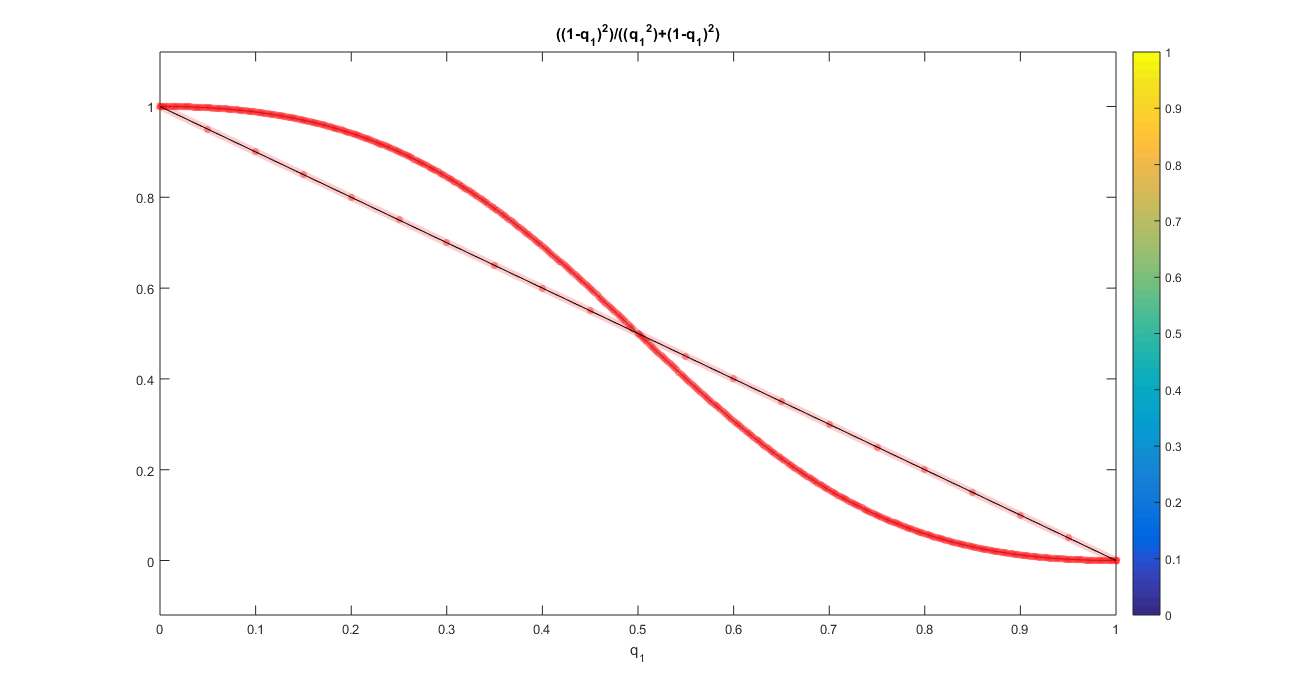
\includegraphics[width=90mm]{Error_2.png}
	\end{figure}


      %% Don't remove the empty line below.  Compilation will fail.
      
  \end{enumerate}
\end{enumerate}

\section{Feature Selection}
We saw in class that one can use a variety of regularization penalties in linear regression.

$$\hat{w} = \arg \min_w  \quad \|Y - Xw\|_2^2 + \lambda \|w\|_p^p$$

Consider the three cases, $p$ = 0, 1, and 2. We want to know what
effect these different penalties have on estimates of $w$.

Let's see this using a simple problem. 

Use the following data (also provided in matlab format).  Assume the
constant term in the regression is zero, and assume $\lambda=1$,
except, of course, for question (1).  You don't need to write code
that solves these problems in their full generality; instead, feel
free to use matlab to do the main calculations, and then just do a
primitive search over parameter space by plugging in a few different
values. Matlab function fminsearch will be helpful. (\emph{Note:} If you are not familiar with function handles, please review the code from HW 2 or see Matlab documentation.)

\begin{enumerate}
\item $\hat{w}_{MLE} = [0.8891;-0.8260;4.1902]$ 
\item $\hat{w} = [0.8646;-0.8210;4.1218]$ 
\item $\hat{w} = [0.8749;-0.8182;4.1829]$
\item Calculating the values of $\hat{w}$ for 8 cases i.e. permuting a 3x1 vector of 0's and 1's and putting in the values of\\
	w computed in the first part.\\
	We get the minimum values for [1;1;1] since the $L_0$ norm will return 0 thus in that case the value will be equal to $W_{MLE}$\\
	Thhus w is [0.8891;-0.8260;4.1902] and the min value is    3.1078e+03\\

\item 

\item When $\lambda > 0$, we make a trade-off between minimizing the sum of squared errors and the magnitude of $\hat{w}$. In the following questions, we will explore this trade-off further. For the following, use the same data from data.mat.
\begin{enumerate}
\item $0.0061$

\item
\begin{enumerate}
	\item Yes the error doubles because the bias increases in the training data.

	\item Nothing happens

\end{enumerate}

\item $\lambda = 4$

\item $\lambda = 28$

\end{enumerate}
\end{enumerate}


\end{document}
